\documentclass[11pt]{article}
\usepackage[includeheadfoot, top=1.0in, bottom=1.0in, hmargin=1.0in]{geometry}
\usepackage[utf8]{inputenc}
\usepackage{fancyhdr}
\usepackage{url}
\pagestyle{fancy}
\usepackage{setspace}
\usepackage{tabularx}
\usepackage{graphicx}
\usepackage{caption}
\usepackage{subcaption}
\usepackage{hyperref}
\usepackage{multicol}


\lhead{Astronomy Lab II}
\rhead{Spring 2022}
\lfoot{Mead}
\rfoot{Mon 6-9pm}
\cfoot{\thepage}

\begin{document}

\begin{center}
\huge{Lab 3: Spectroscopy}\\ \medskip \Large{February 07, 2022}
\end{center}

%%%%%%%%%%%%%%%%%%%%%%% INTRO %%%%%%%%%%%%%%%%%%%%%%%
\section{Introduction: The Rainbow Connection}
Last lab, we studied the multiwavelength universe and learned that the electromagnetic spectrum extends much further than the visible spectrum.  Not only can we use these different wavelengths of light to see different parts of our Universe, but the light that telescopes receive can also tell us about the motion of astronomical objects and the different chemical elements that make up the source of the light.  The method astronomers use to study the motion and chemistry of stars, galaxies, and clusters is called \textit{spectroscopy}.

\medskip \noindent
But what exactly is a \textit{spectrum}?  Before we look at some examples, use your knowledge from the Multiwavelength Universe lab to \textbf{describe what you think a light spectrum is}.

\medskip \noindent
Recall that last week, we explored how different wavelengths of light behave when passed through a prism. If you need a reminder, here is the applet we used last week: \url{https://javalab.org/en/electromagnetic_waves_around_of_visible_rays_en/}.  Today, we will work to answer the following two questions that you thought about last week.

    \begin{enumerate}
        \item If we sent ``white light'' (an equal mixture of all wavelengths) through a prism, what do you expect the light pattern emerging from the prism to look like? 
        
        \item If we were to shine \emph{starlight} through the prism, what could the resulting light pattern tell us about the star?
        
    \end{enumerate}

%%%%%%%%%%%%%%%%%%%%%%% BLACKBODY %%%%%%%%%%%%%%%%%%%%%%%
\section{Blackbody Radiation}
\textbf{In your lab notebooks, briefly reflect on the following:}
\begin{enumerate}
    \item What does it mean for an object to \textit{absorb} light? What color absorbs all wavelengths of light?
    \item What does it mean for an object to \textit{emit} light?
    \item What does it mean for an object to \textit{reflect} light? What color reflects all wavelengths of light?
    \item What does it mean for an object to absorb or emit a \textit{specific wavelength} of light?
    \item If an apple is the color red, what wavelength(s) of light does it reflect? What wavelength(s) of light does it absorb?
\end{enumerate}
A \textit{blackbody} is an idealized object which perfectly absorbs all wavelengths of light, with no reflection. It also emits light at all wavelengths.
\begin{enumerate}
    \setcounter{enumi}{5}
    \item Why do you think a blackbody is called a ``blackbody"?
\end{enumerate}

%The Planck Spectrum and Wien's Law
\medskip \noindent
The spectrum of a blackbody creates a curve called the ``blackbody radiation curve" (i.e. the light emitted at each wavelength). Though blackbodies are idealized spectra (we will explore the ways spectra are not ideal in the next section), stars and many other objects are frequently approximated as blackbodies, which usually works pretty well. Navigate to \url{https://phet.colorado.edu/sims/html/blackbody-spectrum/latest/blackbody-spectrum_en.html}. Check the boxes for ``Graph Values" and ``Labels".  You can use the slider on the thermometer to the right to change the temperature of your test object.  If you need to adjust the size of your graph to see the values, you can use the zoom buttons on each axis.

\medskip \noindent
\textbf{In your lab notebook, make a table with columns for temperature, peak wavelength (the wavelength at which the spectral power density is highest), color, and peak spectral power density.}
\begin{enumerate}
    \item Test at least 6 different temperatures across the full range of the thermometer and fill out the columns in your table.  Please convert your wavelengths to \textit{centimeters}.  For the color column, note which part of the EM spectrum the peak wavelength falls, and if it falls in the visible part of the spectrum, which color it peaks at.  What color does the Sun peak at?
    \item Qualitatively, how do peak wavelength and peak spectral power density change as the temperature increases?
    \item In words, the units on the spectral power density mean ``energy per time per area per wavelength".  How could this relate to the data we collect from telescopes?
    \item Open an Excel or Google spreadsheet. Plot your data with wavelength on the x-axis and temperature on the y-axis.  Make a second plot of your data with 1/wavelength on the x-axis and temperature on the y-axis. \textit{Please make sure to include these plots in your submission.}
    \item Describe what your plots reveal about the relationship between temperature and wavelength.  Are temperature and wavelength directly or inversely proportional to each other?
    \item Make a new column in your table and calculate the value of the peak wavelength (in centimeters) multiplied by the temperature (in Kelvin). Use two significant figures. (\textit{Hint}: You should find that this number is a constant.)
    \item Are red stars or blue stars hotter?
\end{enumerate}

\medskip \noindent
Congratulations! What you just derived is known as \textit{Wien's Law}, an extraordinarily powerful equation used in astronomy. Because $\lambda_{peak} \times T$ is equal to a constant, when we collect light from a star, we can derive the temperature of a star just by seeing which wavelength its light peaks in. In our H-R Diagram lab, you'll discover what else astronomers can learn from knowing the temperature of a star. For now, we'll continue with spectra.

\begin{figure}[h!]
    \centering
    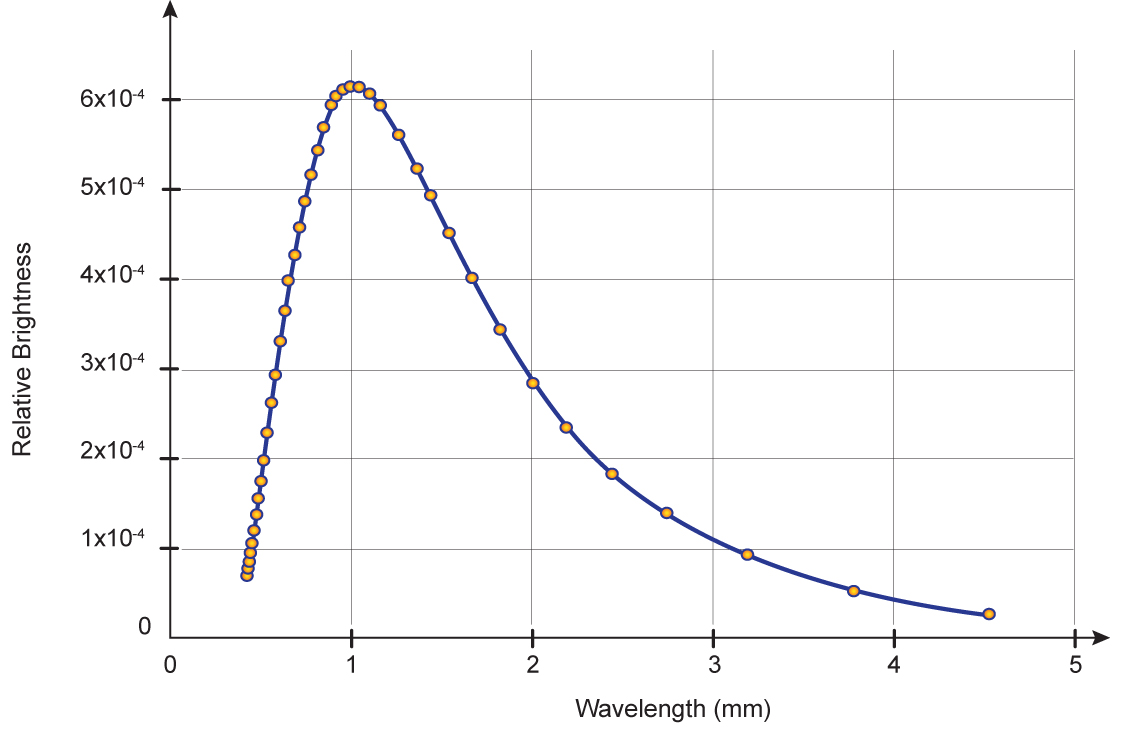
\includegraphics[width=0.7\textwidth]{Images/CMB.jpg}
    \caption{Spectrum of the CMB.}
    \label{fig:CMB}
\end{figure}

\medskip \noindent
One of the most perfect blackbodies in the Universe is called the Cosmic Microwave Background, or CMB for short.  The CMB is the oldest light in the Universe that we can see and comes from the time when the Universe suddenly became transparent to light (you can think of the Universe as a dense, opaque soup before that).  The light of the CMB permeates \textit{everywhere} in the Universe, hence why we call it a ``background".  Since the CMB is a blackbody, we can also estimate its temperature. Figure \ref{fig:CMB} shows the spectrum of the CMB.

\begin{enumerate}
    \item Using Wien's Law, derive the temperature of the CMB.  Watch your units!
    \item Why is the CMB called the Cosmic \textit{Microwave} Background?
\end{enumerate}

\medskip \noindent
The blackbody spectrum is an example of a perfectly smooth spectrum. In reality, stars (and galaxies) have many features and perturbations in their spectra that can tell us much more than just the temperature of the star.  We will explore these next.

%%%%%%%%%%%%%%%%%%%%%%% ELEMENTS %%%%%%%%%%%%%%%%%%%%%%%
\section{Fingerprints of the Elements}

\noindent
Figure \ref{fig:spec} shows examples of two different real spectra.  On the x-axis, we have the wavelength of light.  In general, spectra can cover wavelengths of light across the full electromagnetic spectrum.  On the y-axis, we have \textit{flux}, or the amount of light our telescopes observe. This can be thought of as the number of \textit{photons} our detectors receive per unit time per unit area.  Recall that light can be thought of as either a \emph{wave} (often referred to as an ``electromagnetic'' wave) or as a \emph{particle} (called a ``photon'').  You can think of photons as discrete \textit{packets} of electromagnetic waves that behave like particles, and the more photons of a particular wavelength a telescope collects, the brighter an object is in that wavelength (that is, it has a higher flux in that wavelength).

\bigskip

\begin{figure}[h!]
    \centering
    \begin{subfigure}[b]{0.75\textwidth}
        \centering
        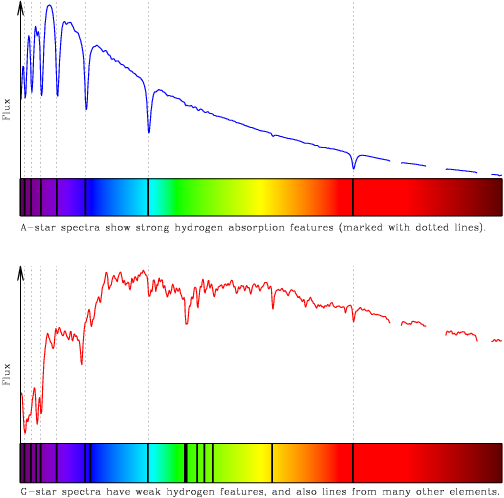
\includegraphics[width=0.75\textwidth,trim={0cm 9.75cm 0cm 0cm},clip]{Images/spectrum.png}
        \caption{A stellar spectrum.}
        \label{fig:stellar_spec}
    \end{subfigure}
    \hfill
    \begin{subfigure}[b]{0.75\textwidth}
        \centering
        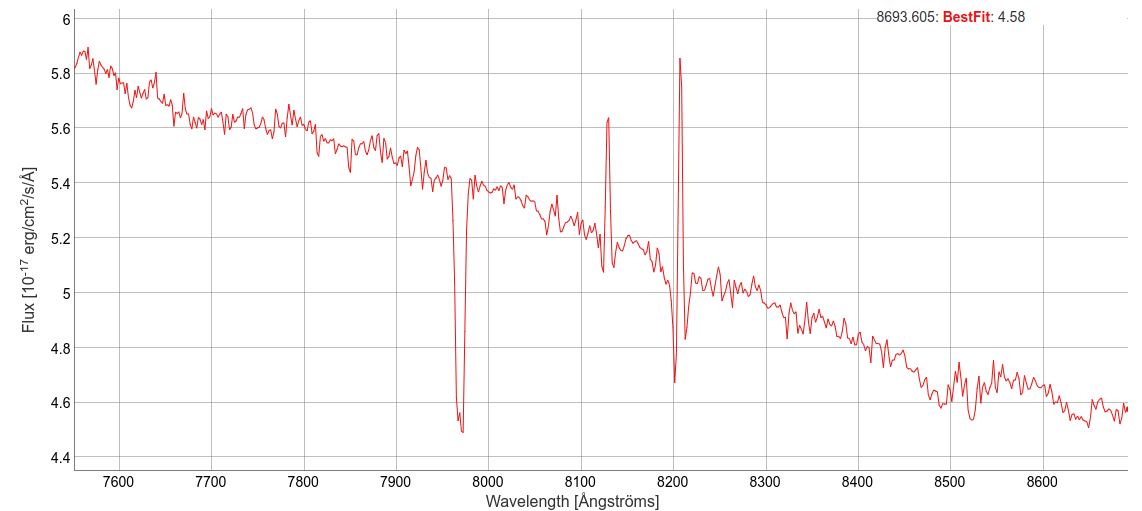
\includegraphics[width=0.75\textwidth,trim={0cm 0cm 0cm 1cm},clip]{Images/gal_spec.png}
        \caption{A galaxy spectrum.}
        \label{fig:gal_spec}
    \end{subfigure}
    \caption{}
    \label{fig:spec}
\end{figure}

\medskip
\begin{enumerate}
    \item Describe some of the features you see in the spectra above.
    \item How do the lines in the lower panel of Figure \ref{fig:stellar_spec} correspond to the upper panel? What do you think might be causing these lines and why?
    \item What do you notice is different between the two spectra? What is similar?
\end{enumerate}

\subsection{Lamp Activity}
%H2, He, N, Ar, Hg, lightbulb

If you do not have one, get a diffraction grating from me.  A \textit{diffraction grating} splits light into it's component colors, much like a prism.  There are 5 lamps set up in the room.  Each lamp is actually heated gas of a specific element.  Go up to each lamp and look at it through your diffraction grating.  \textbf{Make a table in your lab notebook with the element name in the first column and a description of what you observe in the second column.}  Once you have observed each of the lamps, answer the following questions:
\begin{enumerate}
    \item How are each of these spectra similar?
    \item How are they different?
    \item What is your hypothesis about \textit{why} the lamps look different from each other through the diffraction grating?
    \item Which feature of the spectra in Figure \ref{fig:spec} do you think correspond to what you observed?
    \item Now look at one of the light bulbs (a source of white light) in the room with your diffraction grating.  How is the spectrum of the light bulb different from the element lamps?
\end{enumerate}

\begin{figure}[h!]
    \centering
    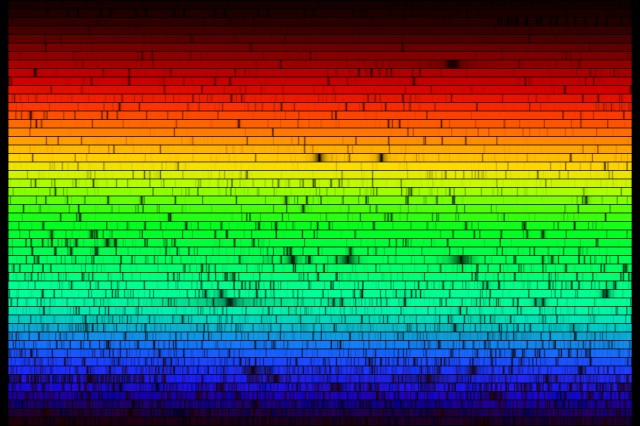
\includegraphics[width=0.7\textwidth]{Images/sun_spec.jpg}
    \caption{The Sun's spectrum. Note that the spectrum has been broken up to fit in the image.}
    \label{fig:sun}
\end{figure}

\noindent
Now check out Figure \ref{fig:sun}.
\begin{enumerate}
    \setcounter{enumi}{5}
    \item How is the Sun's spectrum different from the lamp spectra and light bulb spectrum?
    \item Which feature of the spectra in Figure \ref{fig:spec} do you think correspond to the dark lines in the Sun's spectrum?
\end{enumerate}


\noindent
Figure \ref{fig:types} shows three different types of spectra and how they are formed. Blackbodies emit across all wavelengths and so have a \textbf{continuous spectrum}. Hot gas is made up of specific elements and when these atoms are heated, they \textit{emit} light at certain wavelengths, and so have an \textbf{emission spectrum}.  This emission occurs when an atom's electron moves from a higher energy state to a lower energy state (loses energy).  Since these transitions can only happen at very specific energies, or wavelengths, we see discrete peaks in the spectrum.  You can think of the possible energies of an electron like steps on a staircase.  You can step on each step that is there, but you can't step only half way up or down a step. And the lower on the staircase you get, the less energy you have.  On the other hand, if the light from a blackbody, or continuous spectrum passes through a cool gas that is made up of specific elements, these elements absorb light, and so we get an \textbf{absorption spectrum}. When atoms absorb light, an electron moves from a lower energy state to a higher energy state, or up the staircase. Again, because only very specific photon energies, or wavelengths, can cause these transitions, elements absorb light at the same wavelengths they emit light.  Every atom and molecule has a unique set of electron energy transitions, and thus much like our own fingerprints, a spectral fingerprint that is unique.

\begin{figure}[h!]
    \centering
    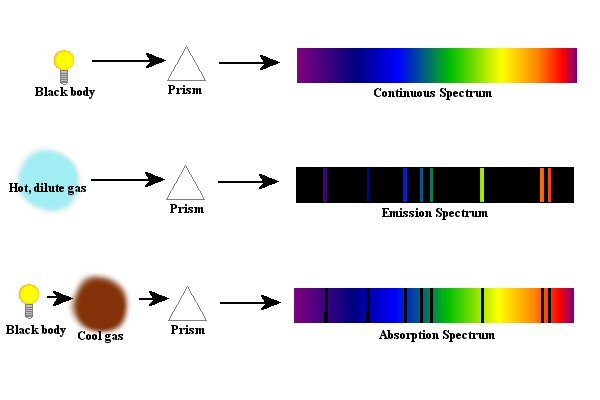
\includegraphics[width=0.9\textwidth,trim={0cm 2cm 0cm 1cm},clip]{Images/emission_v_absorption.jpg}
    \caption{Types of Spectra}
    \label{fig:types}
\end{figure}

\noindent
\textbf{What type of spectrum is:}
\begin{enumerate}
    \item The Sun's spectrum?
    \item The light bulb spectrum?
    \item The lamp spectra?
\end{enumerate}
\noindent
\textbf{Why do you think the Sun has this particular type of spectrum?}

\medskip \noindent
You'll notice that the spectra in Figure \ref{fig:spec} look very different from Figures \ref{fig:sun} and \ref{fig:types}.  Both types of spectra have wavelength on the x-axis, so using what you know about flux, answer the following question:
\begin{enumerate}
    \item How do you think we can translate from the type of spectra in Figures \ref{fig:sun} and \ref{fig:types} to the type of spectra in Figure \ref{fig:spec}? \textit{Hint}: Think about what it would look like for us to receive more or fewer photons of each wavelength in our telescope.
    %\item What does the height of an emission line or the depth of an absorption line mean in terms of how \textit{much} of an element there is along the line-of-sight?
\end{enumerate}

\subsection{Decomposing the Stars}
The spectral fingerprints we just explored are how astronomers are able to pull apart the chemical composition of a star.  If we see an absorption line that we know is from Carbon, then we know that there must be Carbon in the star. The deeper the Carbon absorption line in the spectrum, the more Carbon there must be.

\medskip \noindent
You should have one worksheet and a set of slips: The worksheet should have spectra for seven different elements and the slips should be 5 stellar spectra. Try to identify which elements are in each stellar spectrum by lining them up with the spectra of each element. \textbf{In your lab notebooks, make a table and record which elements you find for each stellar spectrum and then answer the following questions.}
\begin{enumerate}
    \item Which elements are in every star?
    \item Which elements are not in every star?
\end{enumerate}
%\url{https://mrmacha.weebly.com/uploads/5/0/3/9/50390227/star_emission_spectrum_ws.pdf}
%Navigate to \url{https://gizmos.explorelearning.com/}.  Log in using username: astrun1904S22 and password: astronomy. Click on the "Star Spectra" link under "Recently Viewed" and then click "Launch Gizmo".


%%%%%%%%%%%%%%%%%%%%%%% REDSHIFT %%%%%%%%%%%%%%%%%%%%%%%
\section{Oneshift, Twoshift, Redshift, Blueshift}
%Redshift and Blueshift

One of the amazing things about spectra is they can tell us not only about the composition of an astronomical object, but also how far away that object is! We can figure this out through a phenomenon called the \textit{Doppler Effect}.  Much like how the pitch of an ambulance changes as it moves towards you and then away, light does something very similar.  As a source of light moves towards you, the wavelengths of light it emits get compressed, and we see a shorter wavelength than was originally emitted by the star.  This is called blueshift. \textbf{Can you guess why?}  Similarly, if a source of light is moving away from you, the wavelength of light it emits in your direction get stretched, and we see a longer wavelength than was originally emitted by the star. This is called redshift. Check out \url{https://javalab.org/en/doppler_effect_and_redshift_en/} to see how this works. Figure \ref{fig:redshift} shows how the spectra of a redshifted or blueshifted object would look relative to the stationary frame.

\begin{figure}[h!]
    \centering
    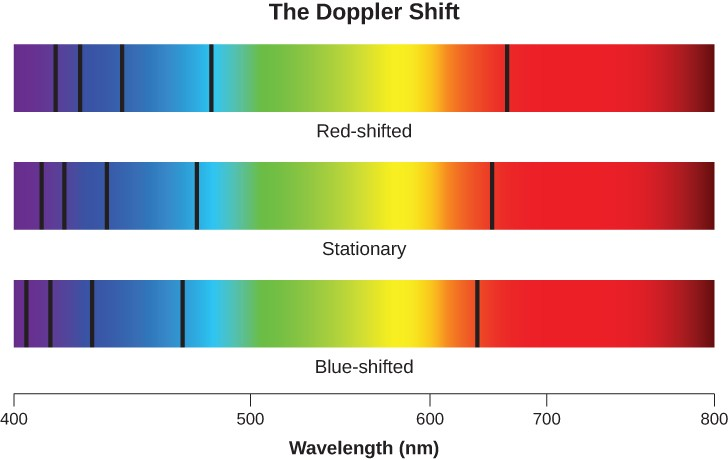
\includegraphics[width=0.75\textwidth]{Images/redshift.jpg}
    \caption{Redshift vs. Blueshift}
    \label{fig:redshift}
\end{figure}

\medskip \noindent
Because the Universe is expanding, most objects, like galaxies for example, are moving \textit{away} from us. Astronomers generally refer to the Doppler Effect on light as ``redshift" because of this, but of course, there are a few objects out there that are instead blueshifted because they are coming towards us. What this shifting of light means for us is that the lines from element spectra \textit{no longer appear at the same wavelength as for a stationary object}.  When light from an object is redshifted, the lines in its spectrum move more towards the red part of the spectrum.

\medskip \noindent
You can calculate the redshift (z) of an object using the following equation:
\begin{equation} \label{eq:redshift}
    z = \frac{\lambda_{obs}-\lambda_{rest}}{\lambda_{rest}}
\end{equation}
\noindent
where $\lambda_{obs}$ is the wavelength of the light we observe with our telescopes, and $\lambda_{rest}$ is the wavelength of light that was originally emitted by the source.

\medskip \noindent
Now, you will get to work with real galaxy spectra from the Apache Point Observatory Galactic Evolution Experiment (APOGEE) survey! Go to \url{https://dr17.sdss.org/optical/spectrum/view}.  Use the search parameters I provide in Table \ref{tab:apogee} to find each of the objects. Once you have input the search parameters, click ``view". On the bottom of the page, you should see a spectrum plot.  You should turn off ``Flux", and turn on ``Smooth".  The vertical lines you see highlight different absorption (red) and emission (blue) features in the spectra.  You can zoom in on a region of the plot by clicking and dragging your mouse along the x-axis. You can zoom out by double clicking. If you hover your mouse over a spectral feature, you can see the wavelength (in Angstroms) in the upper right.

\medskip \noindent
These spectra  are not yet corrected for redshift, and so you'll note that the spectral lines are in different places for different spectra.  Your job is to use a few of these lines to calculate how redshifted each of the spectra are using Equation \ref{eq:redshift}. Table \ref{tab:elements} gives the rest frame wavelength, $\lambda_{rest}$, for some prominent features in the spectra you will look at.  You should choose at least one, if not more, to calculate the redshift of the object. \textbf{Make a table in your lab notebook and record which line you looked at, the rest wavelength (from Table \ref{tab:elements}), the observed wavelength, and show your calculation for the object's redshift.}


\begin{table}[h!]
\begin{minipage}[t]{0.5\linewidth}
    \centering
    \begin{tabular}{c|ccc}
         Object & Plate & MJD & FiberID  \\
         \hline
         Galaxy 1 & 722 & 52224 & 631\\
         Galaxy 2 & 394 & 51913 & 363\\
         Galaxy 3 & 3146 & 54773 & 640\\
         Galaxy 4 & 2565 & 54329 & 41\\
    \end{tabular}
    \caption{APOGEE search parameters}
    \label{tab:apogee}
\end{minipage}
\begin{minipage}[t]{0.5\linewidth}
    \centering
    \begin{tabular}{c|c}
         Element & Rest Frame Wavelength  \\
         \hline
         H$\beta$ & 4863 \AA \\
         OIII & 4959 \AA \\
         OIII & 5007 \AA \\
         CaH & 3968 \AA \\
         CaK & 3933 \AA \\
         OII & 3727 \AA
    \end{tabular}
    \caption{Rest frame wavelengths.}
    \label{tab:elements}
\end{minipage}
\end{table}

\begin{enumerate}
    \item The APOGEE spectrograph (the instrument that measures spectra) only detects wavelengths in the 4000-9000 \AA \, range. You'll have noticed that not all the lines I provided you are visible in every spectrum.  Why not?
\end{enumerate}

\medskip \noindent
As the Universe expands, galaxies are moving away from us at some velocity (this is known as \textit{recessional velocity}).  We can calculate how fast they are moving away using their redshift.  Use the redshifts that you calculated for the galaxies above and Equation \ref{eq:Hubble} to calculate the recessional velocity of each galaxy.

\begin{equation} \label{eq:Hubble}
    z = \frac{v}{c}
\end{equation}

\begin{enumerate}
    \item What relationship do you notice between the redshift and the recessional velocity?
\end{enumerate}

\section{Conclusions}
\begin{enumerate}
    \item Look back on what you have learned in lab so far and describe 3 different ways astronomers use light to learn about the Universe.
    \item A general law in astronomy is that the further away something is from us, the faster it is moving away. This is known as \textit{Hubble's Law}.  We'll study this in more detail later in the semester.  What does Hubble's Law imply about the relationship between redshift and an object's distance from us?
    \item \textit{Challenge Question:} How could you use the spectrum of a star to get the rotation speed of that star? \textit{Hint}: You can take individual spectra of different parts of the star. You should also think about how the material on the surface of the star is moving relative to the observer.
    \item Now that you have completed 3 labs in class and have gotten a sense for how they are structured - do you have any recommendations for improving the labs?  How can I better prepare you to learn the material?  Is there anything \textbf{you} would like to do in class?
\end{enumerate}

\end{document}
